\chapter{Augmenting Nanomolar High-Throughput Screening with Machine Learning for Compound Optimisation} \label{ch:testing}

Accurately determining the biological activity of a molecule requires compound synthesis and purification followed by the preparation of a solution of known concentration to measure compound activity via an assay. However, compound purification can be time-consuming and costly, bottlenecking the throughput of compound screening. This is a challenge, particularly when exploring large and diverse sets of analogues for an intermediate hit or lead compound in order to derive its structure-activity relationship (SAR).

% not quite connected to the first paragraph
Recent work in developing nanomolar-scale high-throughput chemistry seeks to address this issue \cite{Santarilla2015MerckNanomolar, Perera2018PfizerNanomolar, Gehrtz2022nanomolar}. Adopting techniques from plate-based biological-assay screening, reacting one reagent with a different second reagent in each well of the plate, these approaches enable commonplace medicinal chemistry reactions (e.g., amide couplings and Suzuki reactions) to be conducted in a high-throughput manner with minimal starting material (<300 nmol). Utilising this method at the end of a synthesis route allows high-throughput generation of analogues for SAR exploration. In addition to higher throughput, nanomolar-scale chemistry also reduces costs by lowering solvent usage and conserving advanced intermediates in the synthesis route. 

The drawback, however, is that it is rarely possible to perform purification for reactions conducted at the nanomole scale. The output of these reactions is therefore a mixture of chemical reactants, reagents, and products known as a crude reaction mixture. These reaction mixtures can still be assayed for measuring biological activity, but there will necessarily be additional noise as detected potency will be influenced by variations in reaction yield or interference from the reactants. Nevertheless, nanomolar-scale synthesis combined with biochemical screening of crude reaction mixtures has been exploited for the discovery of potent inhibitors for several kinases \cite{Gesmundo2018nanosar, Gehrtz2022nanomolar}, illustrating the potential of this approach for accelerating hit-to-lead drug design.

A related method for high-throughput synthesis is DNA-encoded libraries (DEL) \cite{GirondaMartinez2021DNALibrary}. By linking small molecule building blocks with DNA fragments before chemically enumerating the building blocks with one another, large and diverse combinatorial libraries can be generated. These libraries can be biochemically screened in crude because potent compounds which bind to the protein target can be identified by their DNA tags using high-throughput sequencing methods. There has been recent success in training ML models on DEL bioactivity screen for hit-finding \cite{McCloskey2020DNALibrary, Lim2022DELCountML} as well as toxicology screening \cite{Blay20221DELTox}, and the success of this approach suggests that applying ML to nanomolar screening data may also be possible.

In this chapter, we investigate the application of ML models on bioactivity data from nanomolar-scale high-throughput screening of crude reaction mixtures against SARS-CoV-2 Mpro. We show that ML models can be trained on this data to identify false negatives within the dataset missed due to experimental noise and that these models can be used to identify novel hits in a prospective virtual screen.

% Such derivatization is preferably achieved toward the end of the synthesis route, to maximize the utility of a single intermediate. This approach can be readily scaled to a plate-based format, where the starting material is reacted with a different second reagent in each well of the plate. Provided there is no interference from the other reagents in the reaction, this significantly increases the speed, reduces chemical waste, and lowers the cost of initial SAR exploration. The plate-based format allows closer integration of chemical and biological experiments but also comes with the limitation that reactions conducted at the nanomole scale are rarely appropriate for purification.

% In collaboration with the London Lab at The Weizmann Institute of Science, we investigated whether we needed compound purification at all for training machine learning bioactivity models by using non-purified compound assays. Focusing on a particular scaffold synthesised with a peptide coupling as the final step, we added the acid and amine reactants directly in solution with the protein to obtain an assay reading from the crude reaction mixture. Skipping the purification step allowed us to quickly screen a library of 300 amines with the same acid in high throughput which we used to train RF and GP models. 

\begin{figure}[!t]
 \centering
 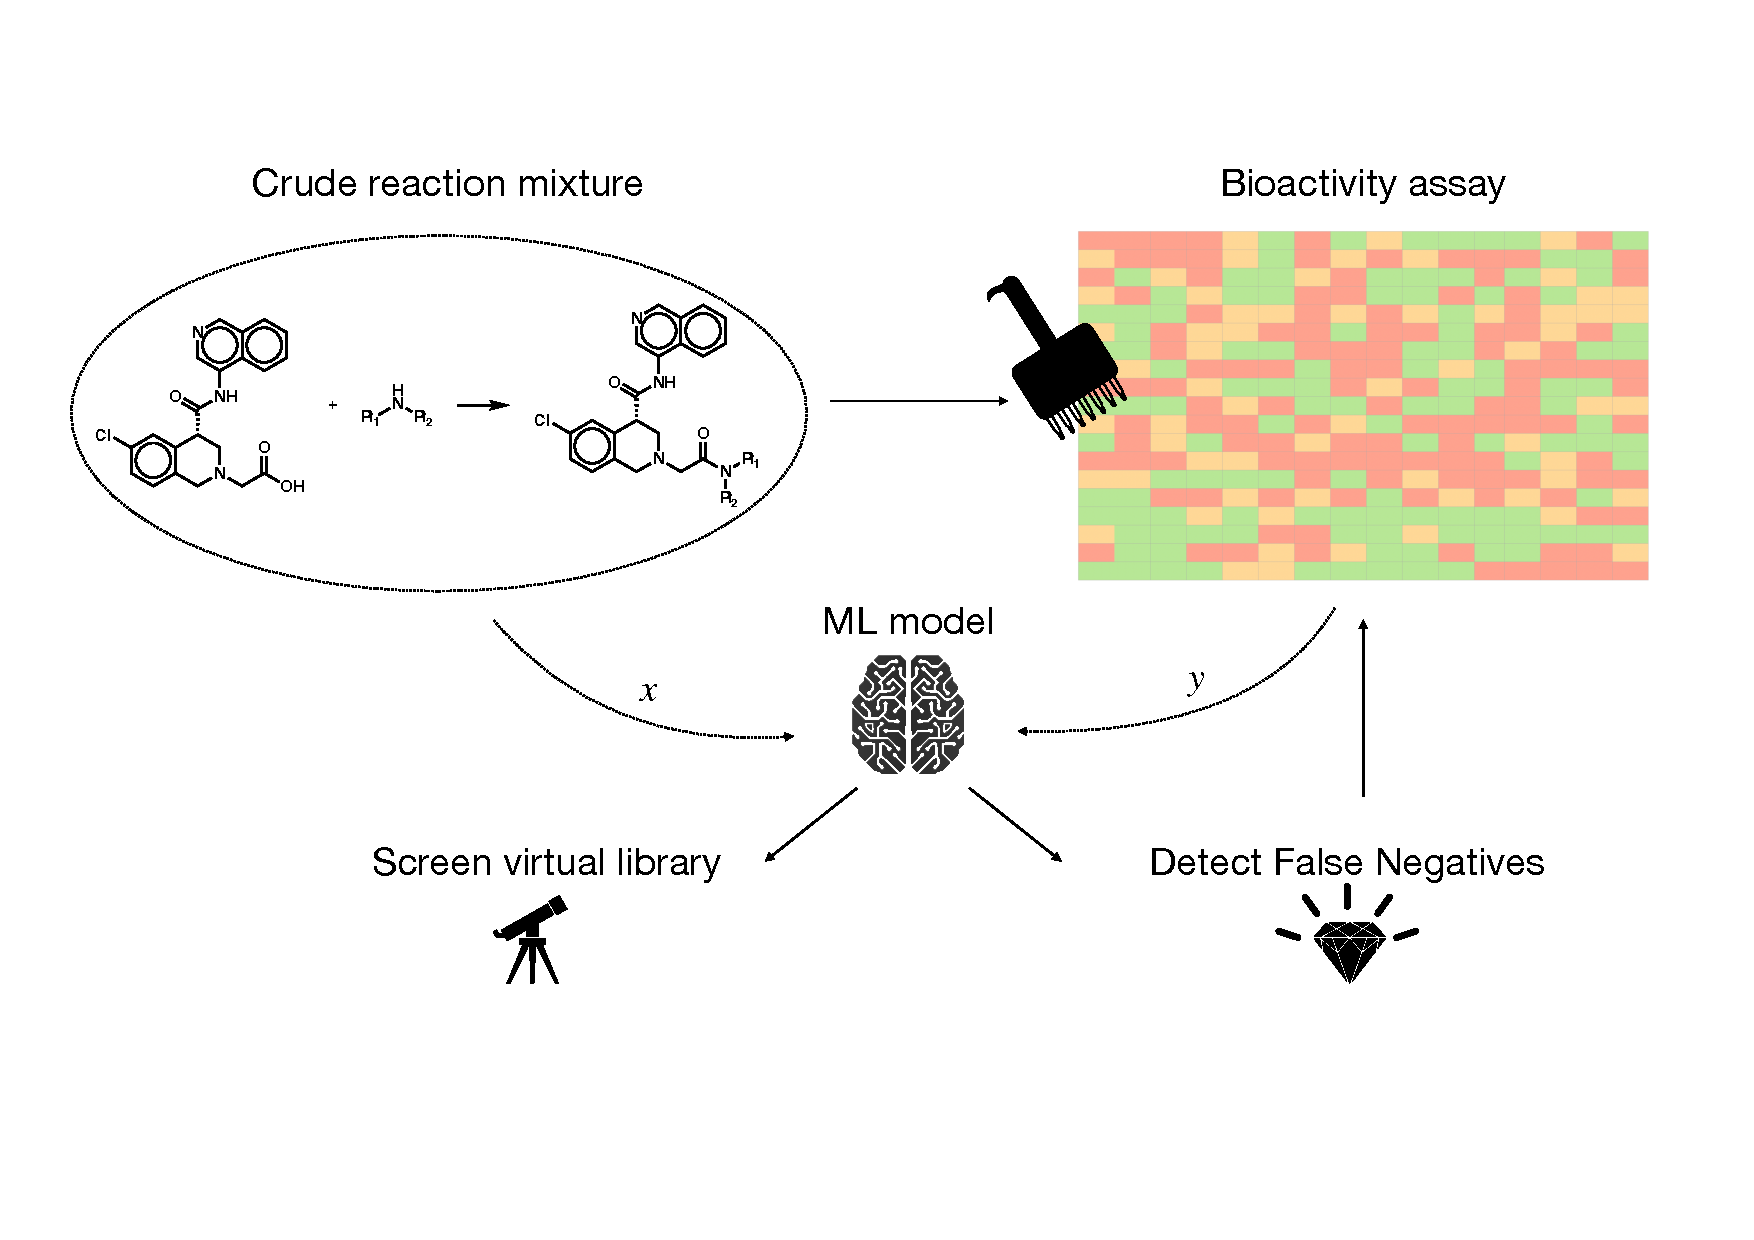
\includegraphics[width=\textwidth]{Chapters/Crude/Figs/schematic.pdf}
 \caption{\textbf{A schematic of the screening workflow.} Nanomolar-scale crude reaction mixtures are assayed for activity against Mpro, and a machine learning model is trained to predict the bioactivity measurements from the chemical structure of the compounds. The trained model is used to identify false negatives in the dataset and to identify novel hits in a prospective virtual screen.}
 \label{fig:schematic}
\end{figure}

\section{Modelling high-throughput crude screening data}

\begin{figure}[!t]
 \centering
 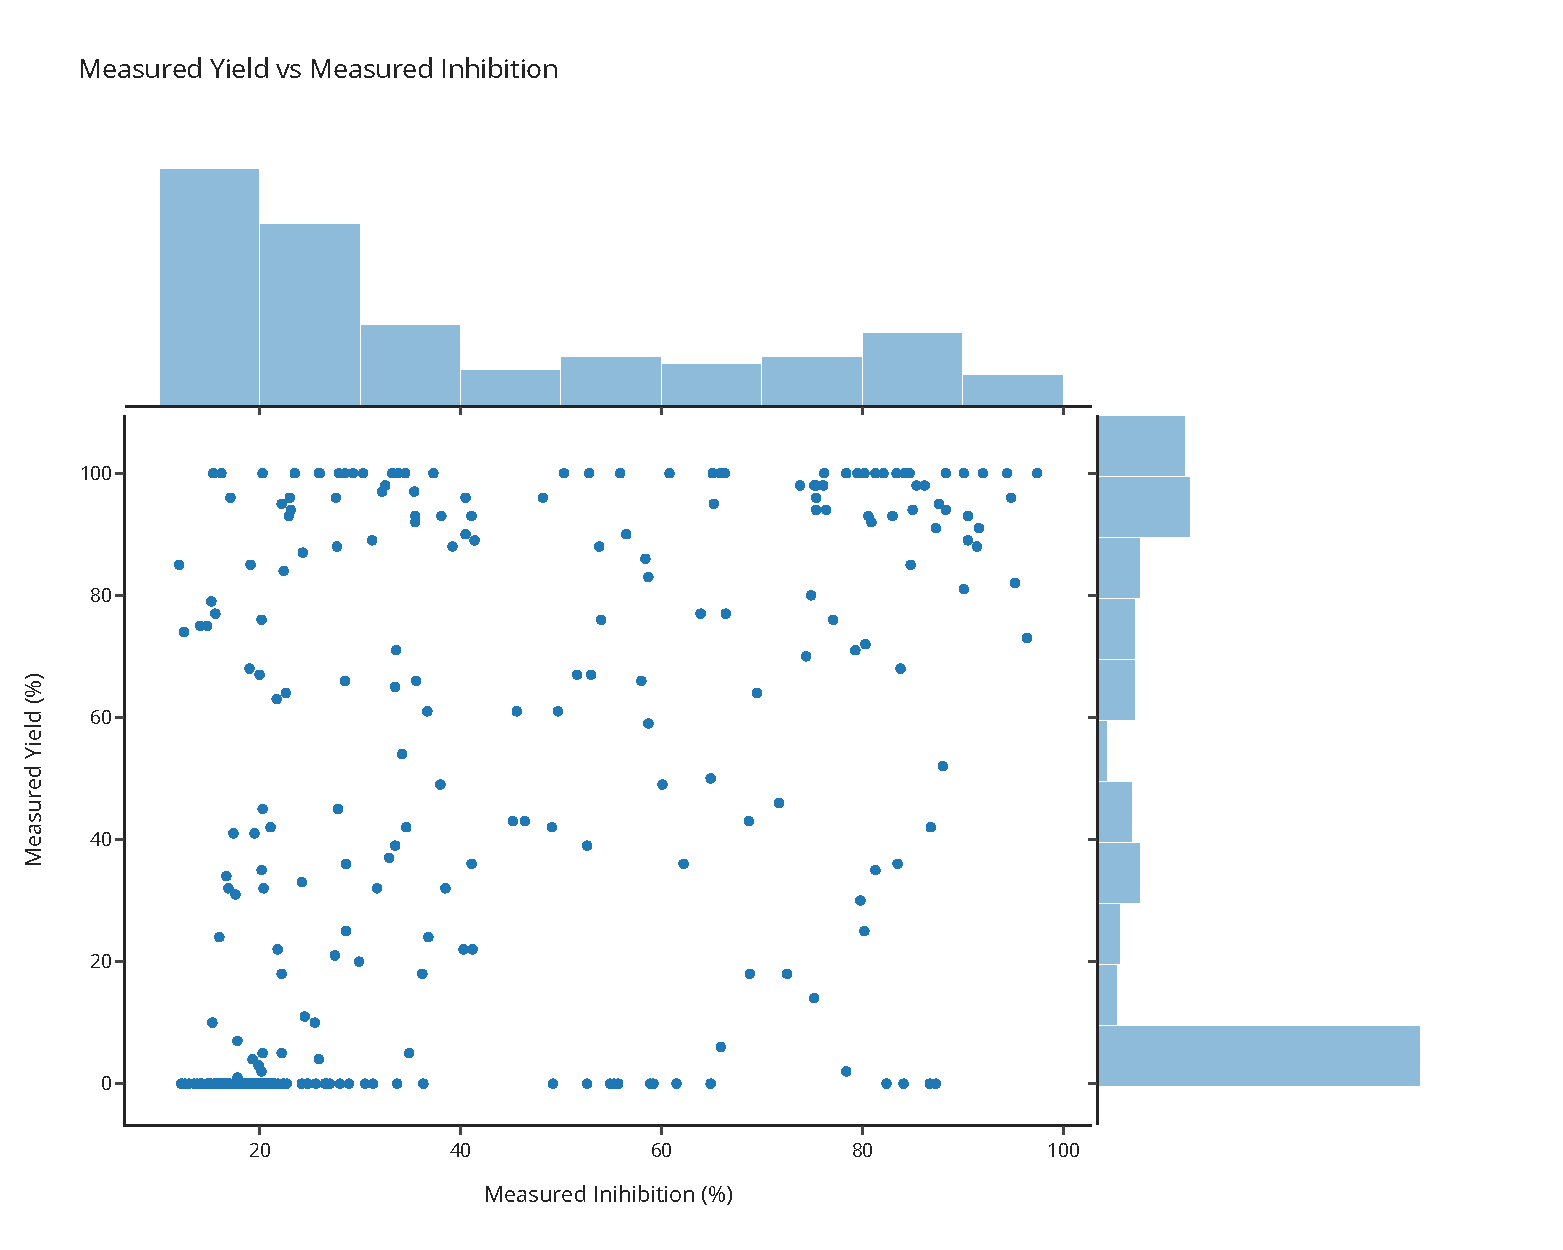
\includegraphics[width=0.85\textwidth]{Chapters/Crude/Figs/yield_vs_activity.pdf}
 \caption{\textbf{The bioactivity of the crude reaction mixtures is influenced by reaction yield.} High-yielding compounds are likelier to exhibit high activity (strongly inhibiting Mpro) while low-yielding compounds tend to have low activity, though the overall correlation is not strong (Spearman correlation $\rho = 0.54$).}
 \label{fig:yield_activity}
\end{figure}

The COVID Moonshot campaign \cite{Moonshot2022} against SARS-CoV-2 main protease (Mpro) investigated multiple chemically diverse molecular series simultaneously in order to minimise the risk of failure. One of the series explored was MAT-POS-4223bc15-21, whose molecular structure had the potential for optimisation towards targeting the P4 pocket of Mpro. 

To rapidly evaluate the SAR of this series, nanomolar high-throughput chemistry was used to enumerate a library of 300 amine building blocks via amide coupling. Yield estimation via integration of UV spectra showed 151 of the library yielded >30\% of the desired product, and the crude reaction mixtures were then assayed against Mpro (Experimental details can be found in Appendix \ref{appendix:mpro_assay} \& \ref{appendix:amide_coupling}).

Although the bioactivity measured in crude is a strong indicator of the potency of compounds, it is also influenced by the yield of the crude reaction mixture. Inspection of the crude activity data reveals a clear relationship (Spearman correlation $\rho = 0.54$) between the measured activity and the yield of the crude reaction mixture (Figure \ref{fig:yield_activity}). Compounds with high yields tend to have strong inhibition, while many compounds with low measured yields have no activity. This means that potentially potent inhibitors may be missed due to low yield from the amide coupling reaction, and this confounding variable adds additional difficulty to the already challenging task of modelling bioactivity with machine learning. 

We model the bioactivity data using two different ML models, taking the mean of their predictions as the final output, to avoid overfitting to the small number of datapoints in this dataset. The two models are: (A) a random forest (RF) model that takes the Morgan fingerprint representation of the amide product in the crude reaction mixture, and (B) a gaussian process (GP) model that takes the Morgan fingerprint representation of the \textit{amine} building block as that is the only varying component in the reactants of the crude reaction mixture. Both models aim to predict the measured activity of the crude reaction mixture.

\begin{figure}[!t]
 \centering
 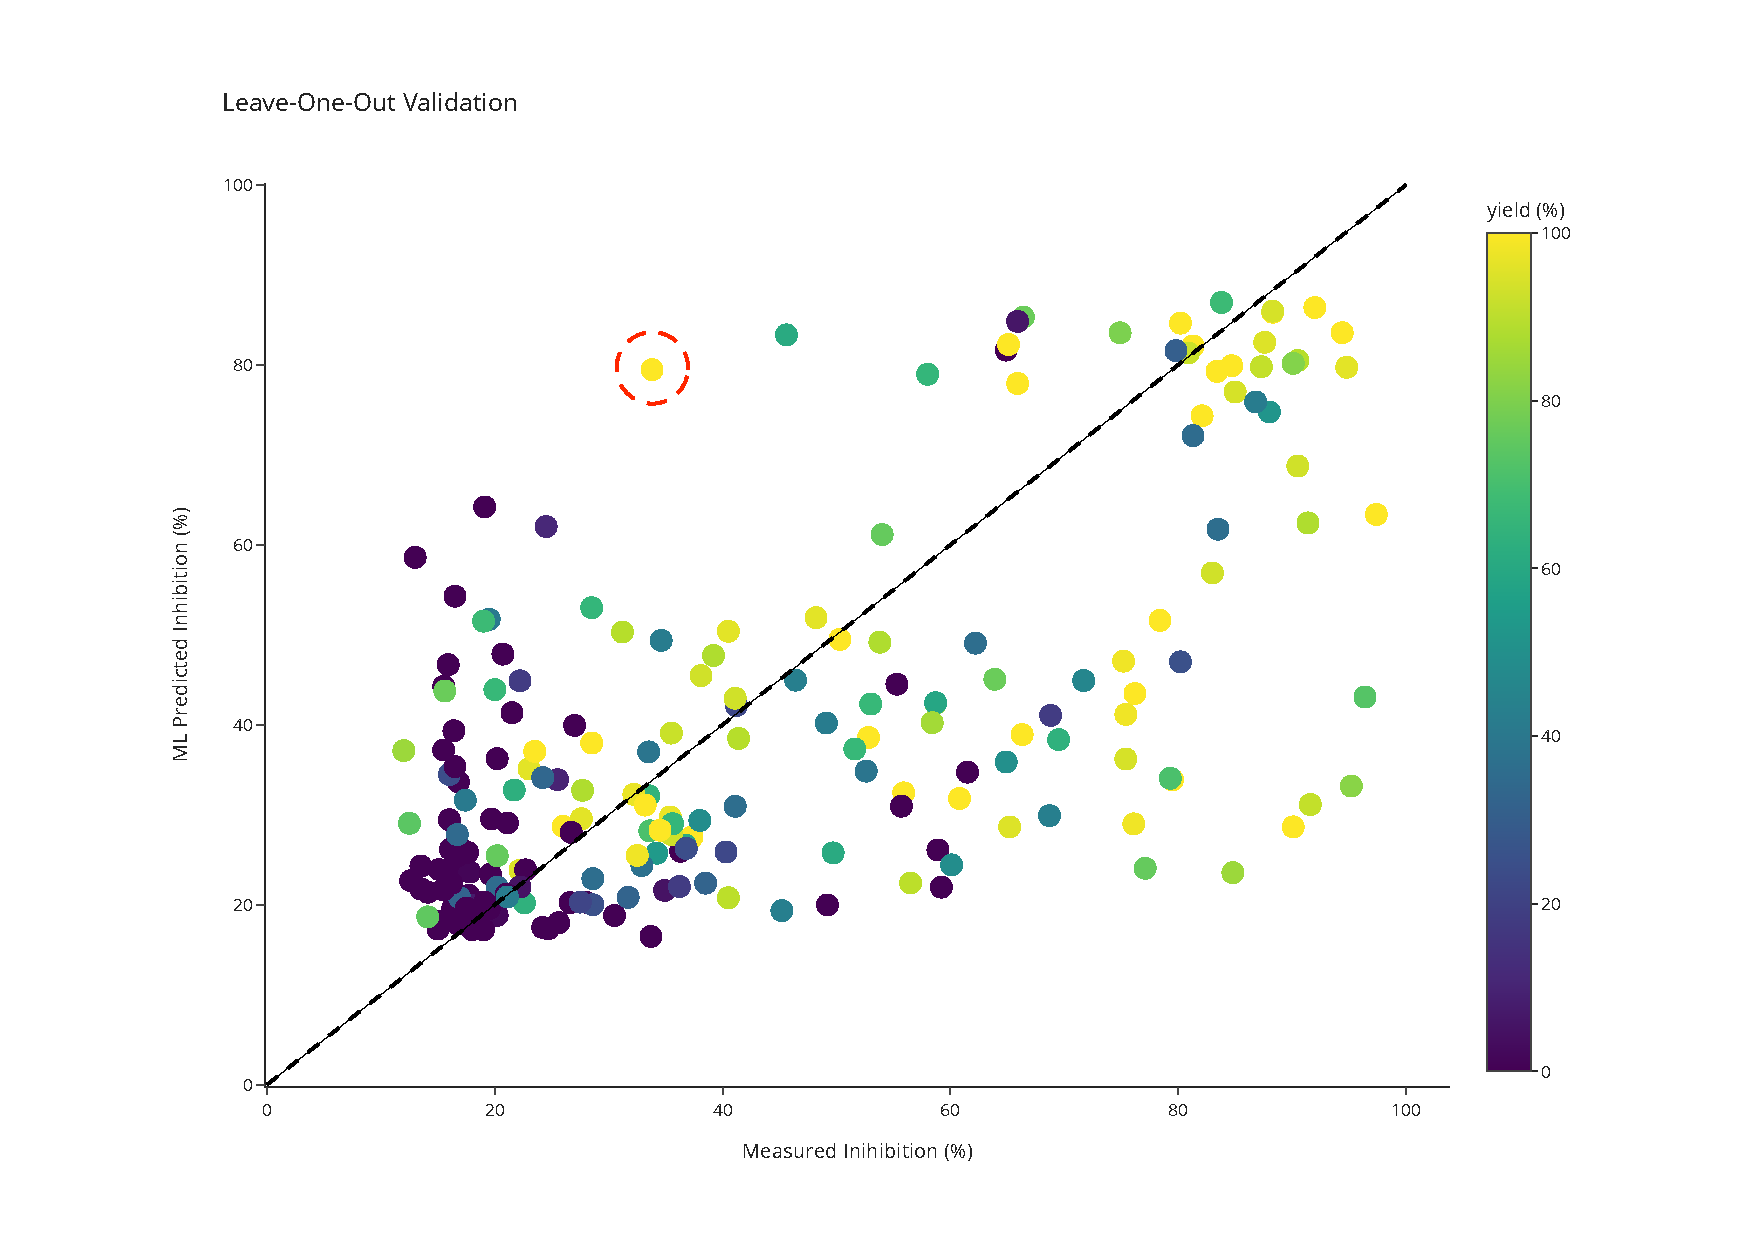
\includegraphics[width=0.85\textwidth]{Chapters/Crude/Figs/rf_loo_flat.pdf}
 \caption{\textbf{Machine learning is able to model crude bioactivity data.} The model predictions ($y$-axis) are generated in a leave-one-out fashion, where the model is trained on all but one datapoint, and then evaluated on the remaining datapoint which is then repeated for each datapoint in the dataset. The datapoint circled in red is a false negative identified by the model and subsequently experimentally validated (Figure \ref{fig:false_negative}).}
 \label{fig:leave-one-out}
\end{figure}

Due to the small size of this dataset, we also choose to use a leave-one-out cross-validation approach to train the models. This means that the model is trained on all but one datapoint, and then evaluated on the remaining datapoint. This is repeated for each datapoint in the dataset (Figure \ref{fig:leave-one-out}). Overall, the model predictions moderately correlate with the experimental measurements (Spearman correlation $\rho =0.64$) and identify distinct clusters of high and low-activity compounds. 

While the model is generally quite conservative in its predictions, it does identify several compounds with a high predicted activity that are not active in the crude assay. We suspected that these were false negatives due to either the low yield of the crude reaction mixture or some other form of experimental noise. We identified 5 compounds with the largest positive difference between predicted and measured activity and re-synthesized, purified and re-tested them with full dose-response curves to obtain IC50 inhibition values. This revealed that one of them was indeed potent with IC50 = $0.113\pm0.046$\uM (ASAP-0000204) (Figure \ref{fig:false_negative}).

% discuss false positives?

\begin{figure}
 \centering
 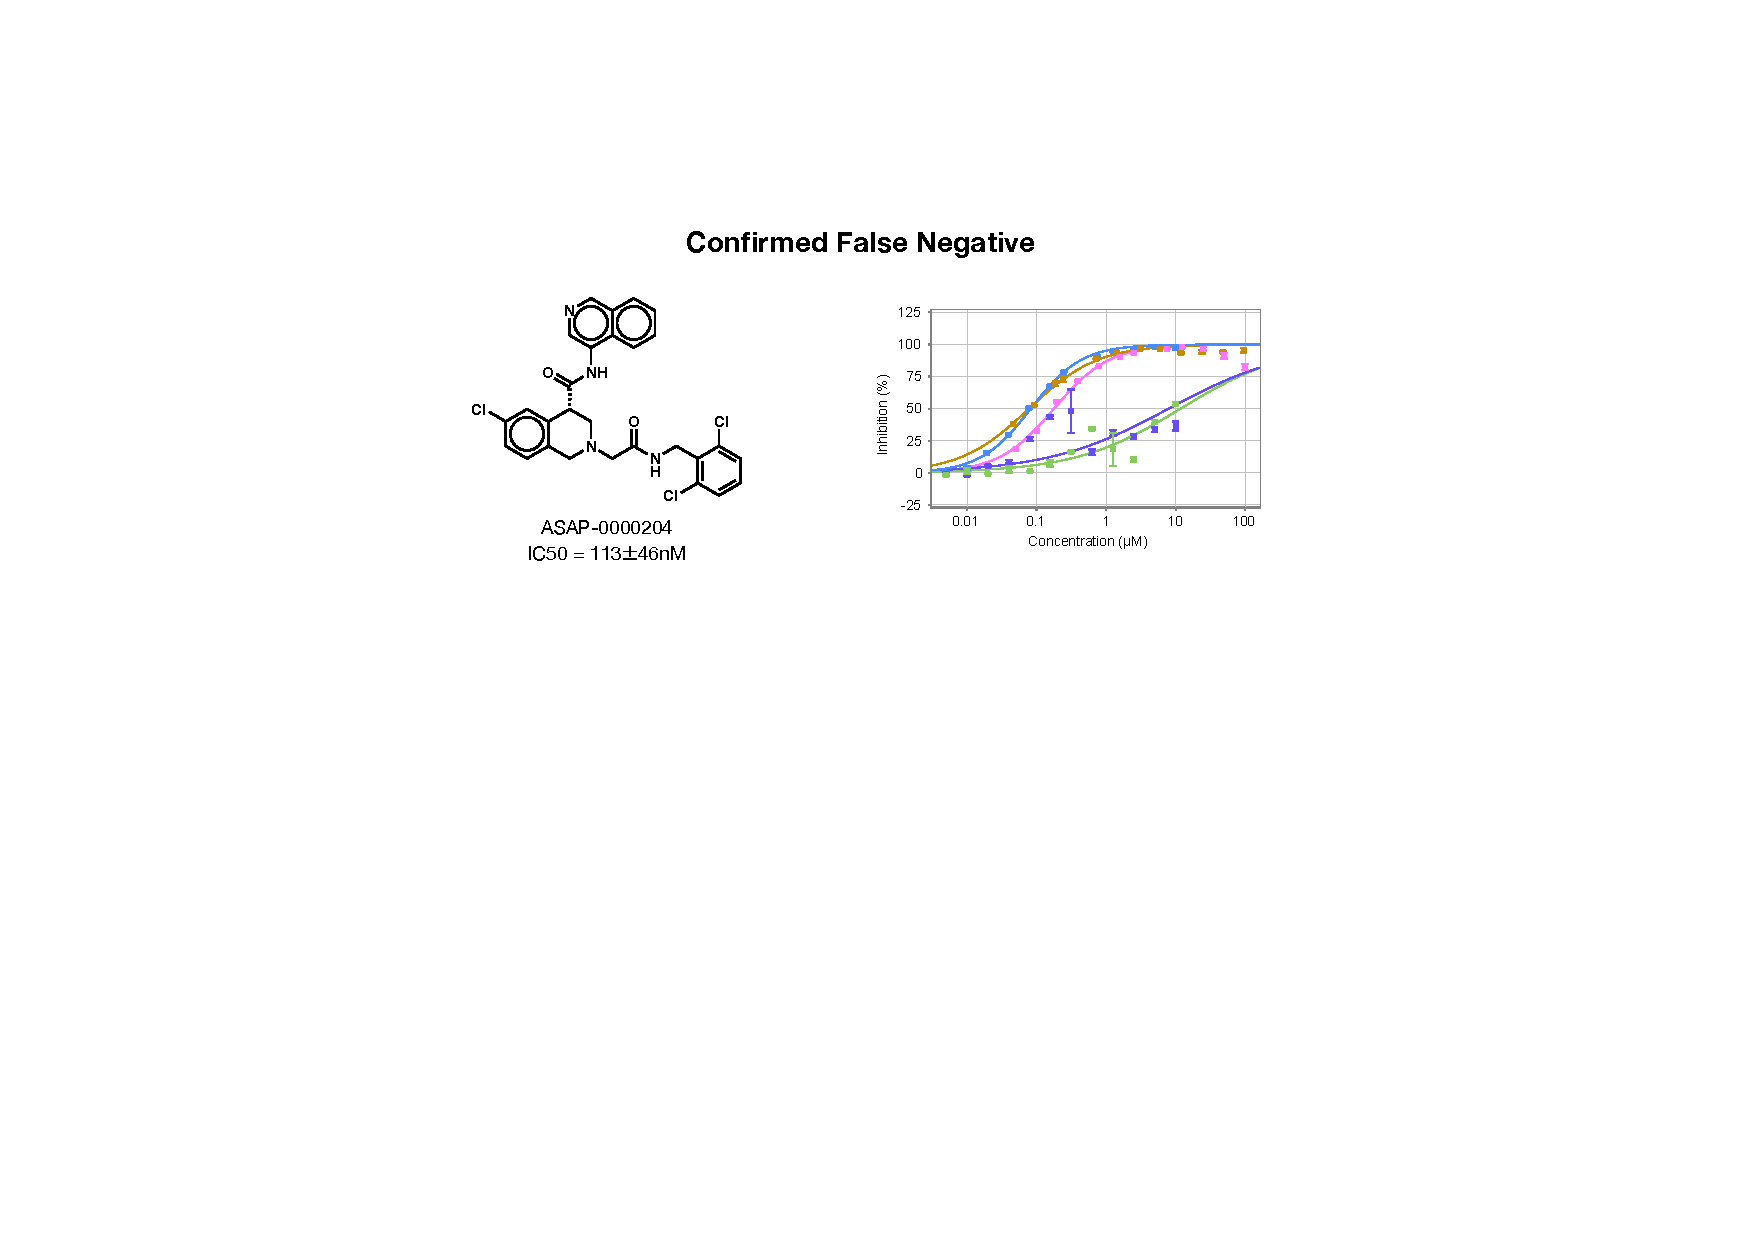
\includegraphics[width=\textwidth]{Chapters/Crude/Figs/false_negative.pdf}
 \caption{\textbf{Experimental validation of ML identified false negative.} A compound with a large positive difference between predicted and measured activity (Figure \ref{fig:leave-one-out}) was re-synthesized and assayed to obtain full dose-response curves. Two sets of curves were obtained with one set demonstrating significantly higher potency than the other, suggesting that solubility issues were interfering with the assay measurements. Examining the higher potency dose-response curves show that the compound has IC50 = $0.113\pm0.046$\uM, which would place it among the top 20 potent compounds in the original dataset.}
 \label{fig:false_negative}
\end{figure}

\section{Prospective Virtual Screening}

Having demonstrated that our ML model can meaningfully learn insights from crude activity data and identify false negatives, we further investigate whether it can extrapolate to novel compounds and be used for virtual screening. The ultimate aim of the SAR exploration of MAT-POS-4223bc15-21 is to optimise potency, and by virtually screening commercially available amine building blocks for the amide coupling reaction we may be able to identify novel compounds with even higher potency.

We construct the screening library by virtually enumerating primary and secondary amine building blocks from Enamine with the same carboxylic acid substructure from MAT-POS-4223bc15-21, resulting in a library of 62,814 amides. These compounds were then filtered for structural alerts and molecules with more than one chiral center were removed to avoid complications in assessing potency. This leaves 58,082 compounds which were scored by the trained GP and RF models, and the top 20 (``ML'') compounds with a high mean predicted activity were selected for synthesis, purification, and assaying to obtain IC50 values.

% TODO - Discuss compounds liked by the model? Discuss structure?

In parallel, the top 20 (``crude'') compounds with the highest measured crude activity from the initial 300 amides were also selected for resynthesis. Crystal structures of the resynthesised compounds bound to Mpro were obtained, verifying that the extended compounds indeed adopt a similar binding mode to the parent, extending towards P3/P5 instead of the P4 pocket nevertheless forming new interactions with Mpro.

\begin{figure}[!]
 \centering
 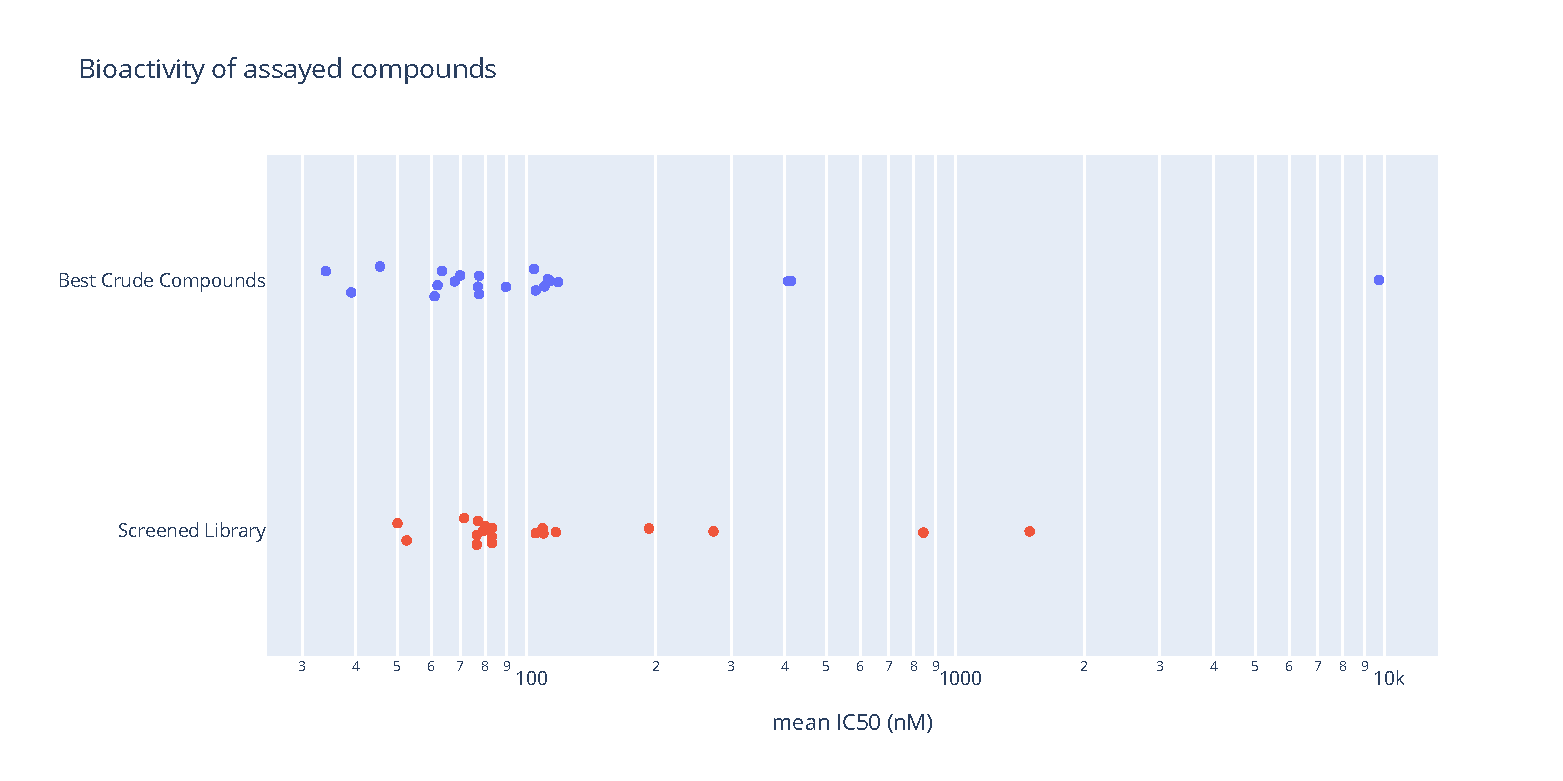
\includegraphics[width=\textwidth]{Chapters/Crude/Figs/strip_plot.pdf}
 \caption{\textbf{The bioactivity distribution of ML-identified compounds from virtual screening is similar to those from the most potent crude compounds.} The top 20 crude compounds are shown in blue, and the top 20 ML compounds are shown in orange.}
 \label{fig:strip}
\end{figure}

\begin{figure}[!t]
 \centering
 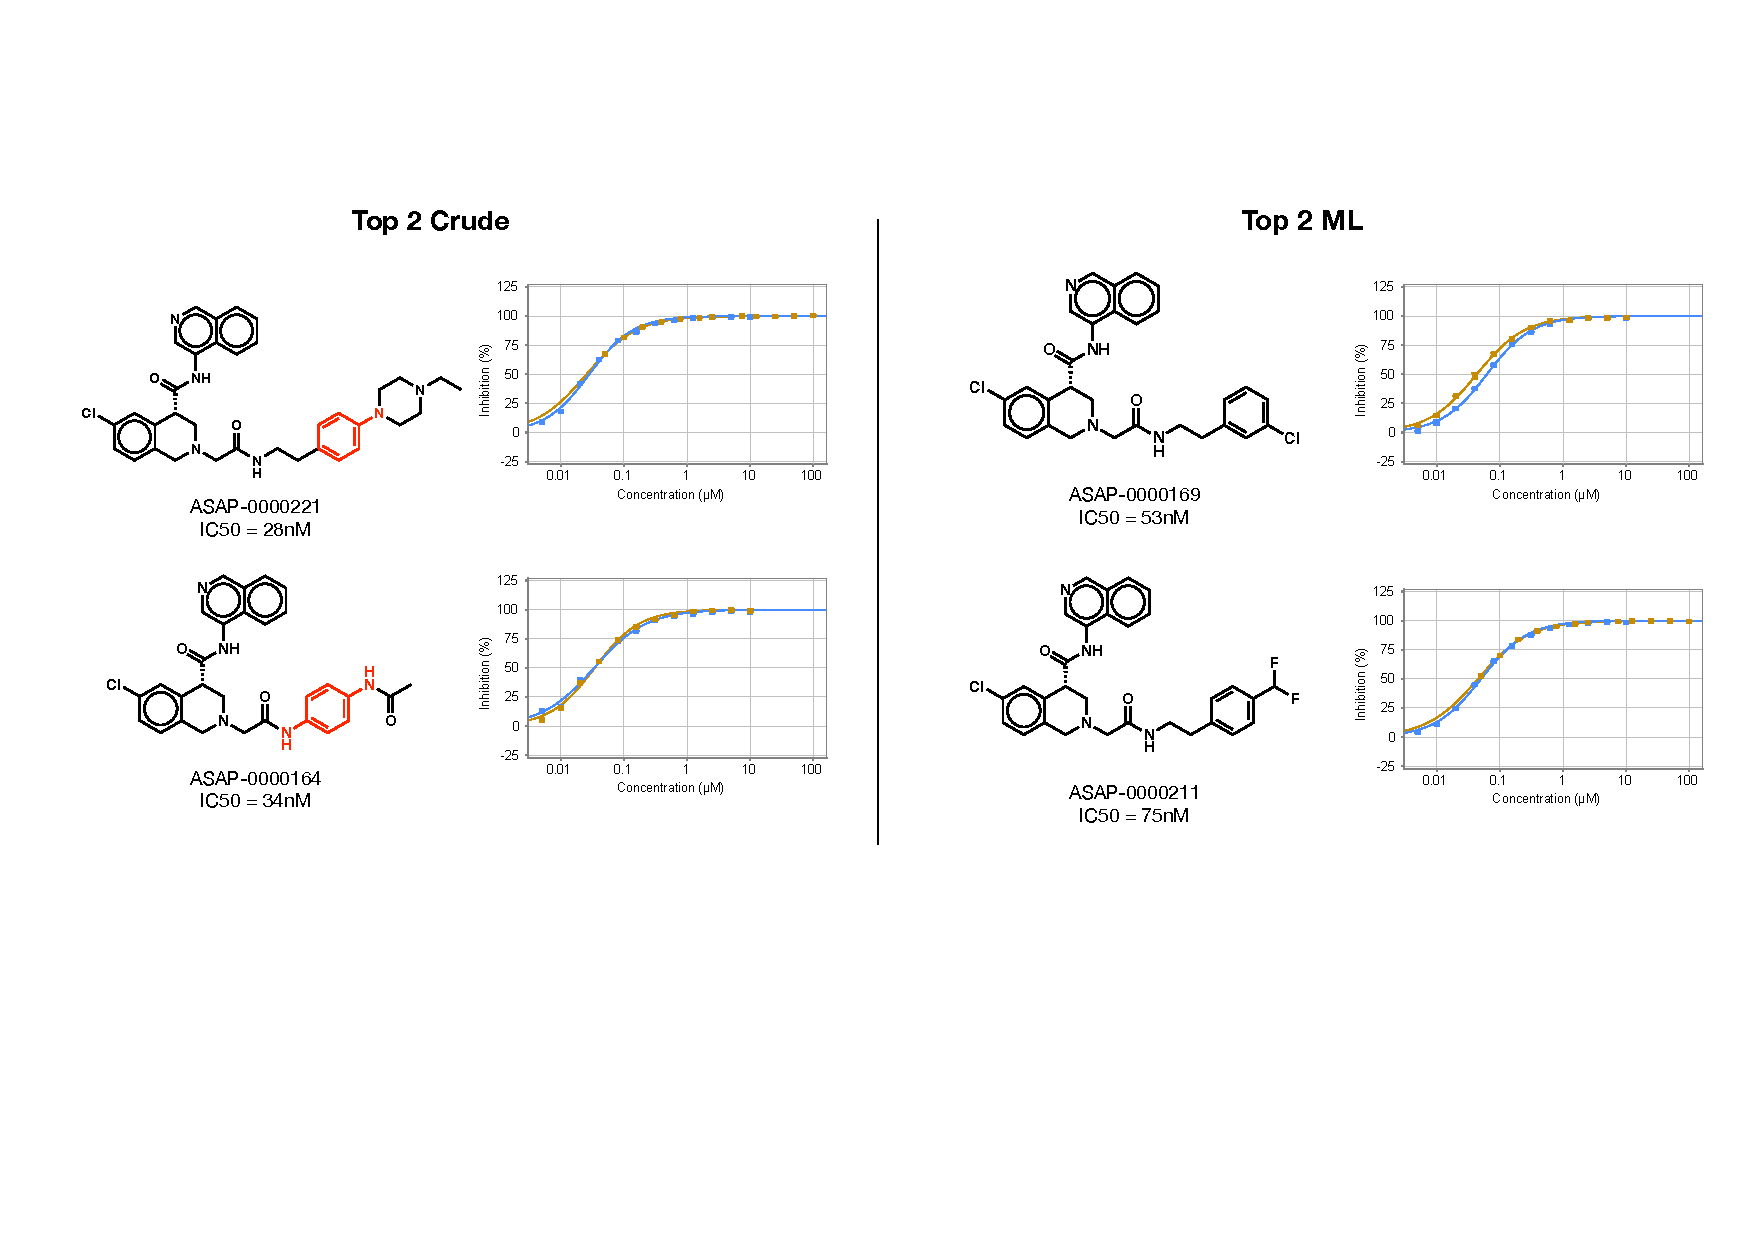
\includegraphics[width=\textwidth]{Chapters/Crude/Figs/ml_vs_crude.pdf}
 \caption{\textbf{Comparison of top ML compounds vs top crude compounds.} The top compounds from the crude screening are more potent but contain aniline motifs (highlighted in red) that are undesirable due to toxicity concerns.}
 \label{fig:ml_vs_crude}
\end{figure}

Both sets of compounds exhibit similar distributions in bioactivity (Figure \ref{fig:strip}), with several compounds improving IC50 by up to 300-fold on MAT-POS-4223bc15-21 (up to 3-fold on the corresponding methyl-amide). The top 2 ML compounds showed promising average IC50 values of 53nM (ASAP-0000169) and 75nM (ASAP-0000211), respectively (Figure \ref{fig:ml_vs_crude}). Although the top 2 most potent crude compounds were more potent with IC50 = 28nM (ASAP-0000221) and IC50 = 34nM (ASAP-0000164), they contain aniline motifs that are generally avoided due to their propensity for the formation of reactive metabolites \cite{Stepan2011aniline}. The top 2 crude compounds without the aforementioned motif had IC50s of 46nM (ASAP-0000155) and 64nM (ASAP-0000225), which are similar to the top 2 ML compounds.

This result highlights ML's ability to identify promising yet overlooked scaffolds without compromising potency. 

\section{Discussion}

% false negatives
In this work, we demonstrate the application of ML models on bioactivity data from nanomolar-scale high-throughput screening of crude reaction mixtures and illustrate the potential of this approach for accelerating compound optimisation in drug discovery. Focusing on the SAR exploration of an inhibitor against SARS-CoV-2 Mpro, we show that ML models trained on nanomolar-scale crude screening data can be used to identify false negatives within the dataset missed due to experimental noise. Furthermore, we show that these models can be used for virtual screening of compound libraries and identify novel potent inhibitors.

The combination of nanomolar-scale synthesis with cellular/biochemical screening is a powerful experimental technique that can greatly speed up compound optimisation and has already demonstrated success in the discovery of potent kinase inhibitors \cite{Gesmundo2018nanosar, Gehrtz2022nanomolar}. Despite the relatively high throughput of this technique, the number of compounds that can be screened is still dwarfed by the size of chemical space, intrinsically limiting the degree to which compound potency can be optimised. Not only can machine learning augment this technique by deconvolution of the experimental noise, they fundamentally extend its reach by utilising the data to virtually screen compound libraries and explore chemical space.

While only a single iteration of model training and prospective testing was investigated in this work, it is clear that the combination of ML with nanomolar high-throughput screening could be very effective in an automated decision-making workflow. As discussed in a previous chapter, an automated workflow for the generation of molecular designs could potentially reduce iteration cycle time, require fewer compounds and iterations to produce a candidate, and scale to more programs \cite{Schneider2018AutomatingDrugDiscovery, Coley2020Outlook, Goldman2022ChemicalDesignLevels}. Nanomolar high-throughput screening could be used as the testing step in such a workflow for performing Bayesian optimisation of compound potency \cite{korovina2019chembo}.

More broadly, the concept of using crude reaction mixtures in place of pure compounds in drug discovery is not limited to biochemical assays. Recent work in utilising crude reaction mixtures for crystallographic fragment screening demonstrated approximately 7x saving of reagents and solvents and up to a 4x reduction in time \cite{Baker2020FragementsFromCrude}. The higher throughput of these approaches necessarily results in additional noise, and perhaps the application of machine learning can be used to detect outliers in such data and perform extrapolation also with the ultimate aim of accelerating drug discovery.

